% !TEX program = xelatex
\documentclass{article}
\usepackage{graphicx} % Required for inserting images
\usepackage{amsmath, amsthm, amssymb, amsfonts}
\usepackage{geometry}
\usepackage{array}
\usepackage{tikz}
\usepackage{hyperref}
\hypersetup{colorlinks=true, linkcolor=blue}
\usepackage{xcolor}
\usepackage{longtable}
\usepackage{fontspec}
\theoremstyle{plain}
\usepackage{amsthm}
% Style for core mathematical results
\theoremstyle{plain}
\newtheorem{thm}{Theorem}[section]
\newtheorem{lem}[thm]{Lemma}
\newtheorem{propn}[thm]{Proposition}
\newtheorem{cor}[thm]{Corollary}
% Style for formal definitions and contextual items
\theoremstyle{definition}
\newtheorem{defn}{Definition}[section]
\newtheorem{eg}{Example}[section]
\newtheorem{conj}{Conjecture}[section]
\newtheorem{prblm}{Problem}[section]
% Style for informal or supplementary notes
\theoremstyle{boldremark}
\newtheorem*{rk}{Remark}
\newtheorem*{note}{Note}

\usepackage{eso-pic, xcolor, graphicx}


\newfontfamily{\tamilfont}{Nirmala UI}
\usetikzlibrary{arrows.meta, decorations.pathmorphing, calc, positioning}
% 1. Link the 'nickname' \customzha to your specific file
\newfontfamily{\customzha}[Path = ./]{HindMadurai-Light.ttf}
% 2. Use the nickname to change the font for just that character
\renewcommand{\qedsymbol}{\textcolor{red}{{\customzha ழ}}}
\DeclareMathOperator{\im}{im}
\definecolor{cyan}{HTML}{00FFFF}



\geometry{a4paper, margin=1in}

\title{\textbf{Group action}\thanks{This is a preliminary draft and currently a work in progress.}}
\author{Gowriprakash}
\date{November 2025}

\begin{document}

\maketitle
\section{Action}

Action of an algebraic object on some other is a general construct of which group action is one.
The simplest concept of an action involves one set, $X$, acting on another set $Y$ and such an action is given by a function $A$, from $X \times Y$ to $Y$,
\[
A: X \times Y \to Y
\]
For a fixed $x \in X$, this produces an endofunction $A_x: Y \to Y$, and hence called ``action by $X$'' (i.e., every $x \in X$ correspond to a map from $Y$ to $Y$). In this way the whole of $X$ acts on $Y$. The image of the action, therefore is the union of the image of all the $A_x$ s.
\[
\text{i.e.,} \quad \mathrm{Im}(A) = \bigcup_{x \in X} \mathrm{Im}(A_x)
\]
% Section for the map expression and illustration
Hence one can talk about the map $x \mapsto A_x$, given by the induced function (say $\hat{A}$),
\[ 
    \hat{A}: X \to Y^Y 
\]
\noindent % This removes the indentation for the next paragraph
where $Y^Y$ is the set of all endofunctions on Y (\text{$X^Y$ is the set of all functions from $Y$ to $X$}).\\
\vspace{1pt}
\begin{center}
    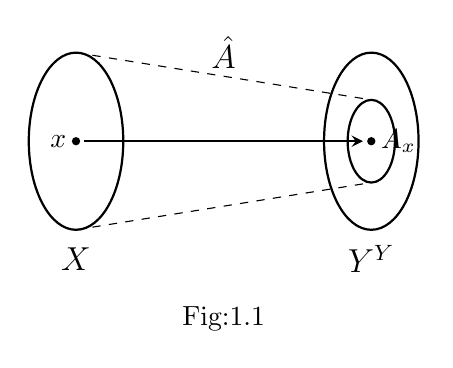
\begin{tikzpicture}[scale=0.75, >=stealth]
        % --- Set X (Domain) ---
        \draw[thick] (0,0) ellipse (0.8cm and 1.5cm);
        \node at (0, -2) {\large $X$};
        \coordinate (x_point) at (0, 0);
        \fill (x_point) circle (2pt) node[left] {$x$};
        \coordinate (x_top) at (0, 1.5);
        \coordinate (x_bottom) at (0, -1.5);

        % --- Set Y^Y (Codomain) ---
        \draw[thick] (5,0) ellipse (0.8cm and 1.5cm);
        \node at (5, -2) {\large $Y^Y$};

        % --- Inner Set (Image) ---
        \draw[thick] (5, 0) ellipse (0.4cm and 0.7cm);
        \coordinate (Ax_point) at (5, 0);
        \fill (Ax_point) circle (2pt) node[right] {$A_x$};
        \coordinate (im_top) at (5, 0.7);
        \coordinate (im_bottom) at (5, -0.7);

        % --- Mapping Arrow (Solid) ---
        \draw[->, thick, shorten >=3pt, shorten <=3pt] (x_point) -- (Ax_point);

        % --- Dashed Lines ---
        \draw[dashed] (x_top) -- (im_top);
        \draw[dashed] (x_bottom) -- (im_bottom);

        % --- Label A_hat ---
        \node at (2.5, 1.5) {\large $\hat{A}$};
        \node at (2.5, -3.0) {Fig:1.1};
    \end{tikzpicture}
\end{center}
If the map $\hat{A}$ is injective, the corresponding action $A$ is called ``faithful'', and unfaithful otherwise.\\
\\
For a `group action', $X$ needs to be a group $G$, and $\hat{A}$, a {\color{red}{group homomorphism}}.\\
\begin{note}
    The idea here is to carry the algebraic structure of the actor to the object being acted upon.
\end{note}    

\clearpage
\noindent


\noindent
Analogous structures of $Y^Y$ (i.e., the codomain of $\hat{A}$, here called the ``target space")  in different categories of $X$ (actor) and $Y$ (being acted upon): \\
\begin{rk}
Target space structure results from the additional structure we impose on $\hat{A}$. Oftentimes that, $\hat{A}$ is a morphism of the category of the actor. The operation(s) under which the target spaces have these structures are often defined pointwise using the operation(s) of $Y$.
\end{rk}
\
\begingroup 
\renewcommand{\arraystretch}{2.2} 
\begin{longtable}{|c|c|c|c|c|} % Changed p{3.5cm} to c for consistency
\hline
\textbf{Category of $X$} & \textbf{Category of $Y$} & \textbf{Target Space} & \textbf{Structure} & \textbf{Formal Name} \\ \hline

$\mathbf{Set}$\footnote{category w/ sets as objects and functions as morphisms} & $\mathbf{Set}$ & $Y^Y$ & Monoid & Action \\ \hline

{\color{red}$\mathbf{Grp}$}\footnote{category of groups and group homomorphisms} & {\color{red}$\mathbf{Set}$} & {\color{red}$\mathrm{Sym}(Y)$} & {\color{red}Group} & {\color{red}Group Action} \\ \hline

$\mathbf{Grp}$ & $\mathbf{Vect}$\footnote{category of vector spaces and linear maps} & $\mathrm{GL}(V)$ & Group & Group Representation \\ \hline

$\mathbf{Ring}$\footnote{category of rings and ring homomorphisms} & $\mathbf{Ab}$\footnote{category of abelian groups and group homomorphisms} & $\mathrm{End}(M)$ & Ring & Ring Representation \\ \hline

$\mathbf{Alg}$\footnote{category of associative algebras and algebra homomorphism} & $\mathbf{Vect}$ & $\mathrm{End}(V)$ & Algebra & Algebra Representation \\ \hline
\end{longtable}
\endgroup

\begin{note}
In the III row, GL($Y$) = GL($V$), for $Y$ is a vector space $V$.\\
In the IV row, End($Y$) = End($M$), for $Y$ is an abelian group thought of as a $\mathbb{Z}-$module $M$.\\
In the V row, End($Y$) = End($V$), for $Y$ is a vector space $V$.\\
\end{note}

\noindent
\textbf{Note}: $Y^Y$ is a superset of all other target spaces.\\
\\
\textbf{Irrelevant info}: Notice how action goes along the process of experimentation. A test subject $Y$, being acted upon by a known structure $X$ to comment of the unknown structure of $Y$ based on the interaction (for eg. a scattering experiment).
\\
\section{Group action}
In case of group actions, we add an extra condition on the induced function of the action $A$ (i.e., $\hat{A}$), that it must be a group homomorphism. Let's call this new, more restricted $\hat{A}$ as $\hat{A_G}$. Let's rename $X$ (the actor) as $G$, for it's a group, and $Y$ (the set being acted upon) as $X$, for $Y$ always succeeds $X$ and there's no $X$ to preceed it, so a group action $A_G$ is given by,
\[
\text{$A_G$}: G \times X \to X.
\]
Now, the associated induced function
\[
\hat{A_G}: G \to X^X
\]
needs to be a group homomorphism.\\
\\
\noindent
For a function $\rho :G \to H$ to be a group homomorphism where both $G$ and $H$ are groups, satisfying,
$\rho(gh) = \rho(g)\rho(h)$ for all $g, h\in G$, is enough. Because from this condition alone, $\rho(e_G) = e_H$ is implied,
\clearpage 
\noindent
thanks to the invertibility of $H$. The proof goes, $\rho(e_Ge_G) = \rho(e_G)\rho(e_G) = \rho(e_G) \implies \rho(e_G) = e_H$ solely because $\rho(e_G)$ is an element of $H$, therefore invertible ($e_G$ and $e_H$ are the identities of $G$ and $H$ respectively).\\
\\
But here, $X^X$ (say, $M$) is just a monoid under composition (i.e., elements are not necessarily invertible) which forces us to add the condition $\rho(e_G) = e_M$ ($e_M$ is the identity of the monoid $M$) to ensure invertibility in the image of the map $\rho$ (reasoning in section 2.1), rendering $\rho$ into a group homomorphism.\\
\\
i.e., given $\rho(e_G) = e_M$, $\rho(gg^{-1}) =\rho(g)\rho(g^{-1}) = e_M$ and hence $\rho(g)$ is invertible with inverse $\rho(g^{-1})$for all $g \in G$.\\

\subsection{Basis of homomorphism conditions}
As the name suggests, homomorphisms are the morphisms that morphs objects into the same category, i.e., if the domain is a group, so is the image of a group homomorphism. Let's look at how the conditions $\rho(gh) = \rho(g)\rho(h)$ for all $g, h \in G$ and $\rho(e_G) = e_M$ combinedly ensure this when the codomain is a monoid.\\
\\
$\rho(gh) = \rho(g)\rho(h)$ ensures closure of the image. $G$ is closed $\implies$ $gh \in G$ for all $g, h\in G$ and $\rho(g) \in \text{Im}(\rho)$ for all $g \in G$
$\implies \rho(gh) = \rho(g)\rho(h) \in \text{Im}(\rho)$ for all $\rho(g), \rho(h) \in \text{Im}(\rho)$ 
$\implies \text{Im}(\rho)$ is closed. \\
\\
Associativity is inherited for any non-empty subset of a monoid, since a monoid is associative. \\
\\
Now comes the crucial part. $\text{Im}(\rho)$ being invertible. i.e., for each $\rho(g) \in \text{Im}(\rho)$, there exists $(\rho(g))^{-1}$ such that, $\rho(g)(\rho(g))^{-1} = e_M$. Assume $\rho(e_G) = m \in M$ and $m \neq e_M $ 
$\implies \rho(e_G e_G) = \rho(e_G)\rho(e_G) \implies \rho(e_G) = m^2 \implies m = m^2$ 
$\implies m$ is an idempotent element.\\
\\
Therefore the identity, in itself, has this property of getting mapped to an idempotent elment under the condition $\rho(gh) = \rho(g)\rho(h)$ for all $g, h \in G$.  \\
\\
Now, we also need $m$ to be invertible, for we need Im($\rho$) to be a group. i.e., there exists $ m^{-1} \in Im(\rho)$ such that $m m^{-1} = e_M \implies m  m  m^{-1} = m e_M$ 
$\implies m^2 m^{-1} = m \implies mm^{-1} = m \implies m= e_M \implies \boxed{\rho(e_G) = e_M}$ \\
\\
i.e., the only invertible idempotent element in a monoid is the identity.\\
\\ 
The conditions, $\rho(gh) = \rho(g)\rho(h)$ for all $g, h \in G$ and $\rho(e_G) = e_M$ ensure that Im({$\rho$}) is a group, the associated map $\rho$, a group homomorphism, which is what we wanted the induced map $\hat{A_G}$ of our group action $A$ to be (i.e., a group homomorphism).\\
\\
\\
\\
Now, eventhough the codomain $M$ is a monoid, the image of $\hat{A_G}$ is a group, a subgroup of the monoid $M$. And for any monoid $M$, the subset of units, $M^*$ is a group, and is the biggest subgroup of the monoid to which every other subgroup is a subgroup of. Therefore $Im({\rho}) <$ $M^*$,\footnote{whenever I use, $\subset$ or $<$, the former is an improper subset, the latter, an improper substructure (i.e., subspace of a vector space, subsgroup of a group etc.,) otherwise would be explicitly mentioned, a subgroup of a monoid for example, would be explicitly mentioned. For proper couterparts, i use $\subsetneq$ and $\lneq$ respectively.} and the the group of units $M^*$ of our monoid $M = X^X$ is the set of all invertible endofunctions on $X$, a.k.a. bijections from $X$ to $X$, which is nothing but the symmetric group $S_X$\footnote{$S_X$ is the symmetric group of $X$, Sym($X$)}.
\\
\\
Thus the induced map of a group action $A_G : G \times X \to X $ is
\[
\hat{A_G} : G \to S_X,
\]
which is a group homomorphism.\\

\begin{center}
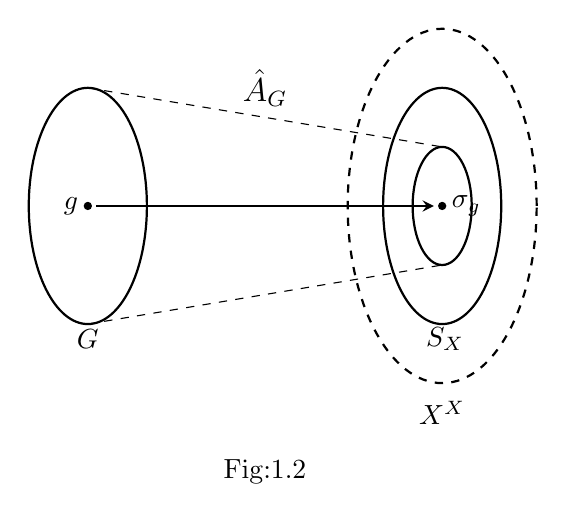
\begin{tikzpicture}[scale=0.75, >=stealth]
    % --- Group G (Domain) ---
    \draw[thick] (0,0) ellipse (1cm and 2cm);
    \node at (0, -2.25) {$G$};
    \coordinate (g_point) at (0, 0);
    \fill (g_point) circle (2pt) node[left] {$g$};
    \coordinate (g_top) at (0, 2);
    \coordinate (g_bottom) at (0, -2);

    % --- Set X^X (Codomain - Larger and Dashed) ---
    \draw[thick, dashed] (6,0) ellipse (1.6cm and 3.0cm);
    \node at (6, -3.5) {$X^X$};

    % --- Set S_X (Symmetric Group) ---
    \draw[thick] (6, 0) ellipse (1.0cm and 2.0cm);
    \node at (6.05, -2.25) {$S_X$};

    % --- Inner Set (Image of G under the homomorphism) ---
    % This is the new, smaller ellipse inside S_X
    \draw[thick] (6, 0) ellipse (0.5cm and 1.0cm);
    % \node at (6, -1.3) {\footnotesize Im($\hat{A}_g$)}; % Optional label for the image

    % --- Point sigma_g (inside the innermost ellipse) ---
    \coordinate (sigma_point) at (6, 0);
    \fill (sigma_point) circle (2pt) node[right] {$\sigma_g$};

    % --- Projection Targets (Top/Bottom of the innermost ellipse) ---
    \coordinate (im_top) at (6, 1.0);
    \coordinate (im_bottom) at (6, -1.0);

    % --- Mapping Arrow ---
    \draw[->, thick, shorten >=3pt, shorten <=3pt] (g_point) -- (sigma_point);

    % --- Projections (Projecting G into the innermost ellipse) ---
    \draw[dashed] (g_top) -- (im_top);
    \draw[dashed] (g_bottom) -- (im_bottom);

    % --- Label for the Map ---
    \node at (3, 2.0) {\large $\hat{A}_G$};
    \node at (3, -4.5) {Fig:1.2};
\end{tikzpicture}
\end{center}
\begin{note}
$\sigma_g$ is a bijection (as any element of a symmetric group) that $g$ is getting mapped to.
\end{note}
Now one can draw analogies from Fig:1.1, that when the actor gets changed from a set to a group, the mapping gets more restrictive, codomain shrinks from $Y^Y$ to $S_X$  (ofcourse, it's because we wanted $\hat{A_G}$ to be a group homomorphism). Since $\hat{A_G}$ preserves group structure, unlike $\hat{A}$ in the case of action by a set.\\
\\
Let's see how this naturally leads us to the axioms of a group action.\\

\noindent For $\hat{A}_G$ to be a group homomorphism, the following must be satisfied:
\begin{align*}
   \hat{A_G}(gh) &= \hat{A_G}(g)\hat({A_G}(h)) \ \text{for all} \ g, h \in G \\
   \hat{A_G}(e_G) &= e_M
\end{align*}
\noindent
Now, $\hat{A}_G$ is a function from $G$ to $S_X$, for 2 functions to be deemed `same' in $S_X$, we need them to be same for every $x \in X$. \\
\begin{align*}
    \text{i.e.,} \quad \hat{A}_G(gh)(x) &= \hat{A}_G(g) (\hat{A}_G(h)(x)) \ \text{for all} \ g, h \in G\  \text{for each} \ x \in X \\
    \hat{A}_G(e_G)(x) &= e_M(x) =x \ \text{for all} \ x \in X
\end{align*}
Since the identity of the monoid $X^X$ or the group $S_X$ is nothing but the identity function (i.e., $e_M(x) = x \ \text{for all} \ x \in X$).\\
\\
\textbf{Note}: ${A}_G(g,x) = \hat{A_G}(g)(x) = \sigma_g(x) $\\
\\
Therefore, the above reads,
\begin{center}
\fcolorbox{black}{white}{
    \begin{minipage}[c][1.25cm][c]{0.55\textwidth}
        \vspace*{\fill}
        \begin{align*}
            A_G(gh, x) &= A_G(g, A_G(h, x)) \ \text{for all}\ g, h \in G\ \text{for each}\ x \in X \\
            A_G(e_G, x) &= x \ \text{for all}\ x \in X
        \end{align*}
        \vspace*{\fill}
    \end{minipage}
}
\end{center}
which exactly are the axioms of a group action.\\
\begin{note}
For notational convenience, $A_G(g,x) = g\cdot x$
\end{note}
\
\begin{thm}[Cayley's theorem]
Every group is embedded in a symmetric group.
\end{thm}
\begin{proof}
The goal here is to show that for every group $G$, there exist a set $X$ on which $G$ acts faithfully. Since for a faithful group action, $\hat{A_G}$ is injective (which already is a group homomorphism), resulting in an embedding of $G$ into $S_X$ (i.e., Im($\hat{A_G}$) is isomorphic to $G$).
The standard proof involves the set $X$ being the group $G$ itself ($X=G$), and the action being left multiplication.
\[
A_G : G \times G \to G \ \text{given by} \ A_G(g,h) = g \cdot h =gh
\]
\begin{note}
Don't confuse the condition as $A_G$ being an injection. It's $\hat{A_G}$ that needs to be an injection, for $A_G$ to be faithful.
\end{note}
\noindent
the endofunction (which is a bijection) defined by a specific $g \in G$ is
\[
A_G(g,h) = \sigma_g(h) \ \text{for all}\ h \in G.
\]
The induced map is
\[
\hat{A}_G : G \to S_G \ \text{given by} \ \hat{A}_G(g) = \sigma_g.
\]
The goal is to show this induced map is injective. In other words, every $g \in G$ correspond to a unique bijection from $G$ to $G$.\\
\\
For this map to be a non-injection, $\sigma_{g_1}(h) = \sigma_{g_2}(h)\ \text{for all}\ h \in G$ for some $g_1, g_2 \in G$. But here, $\sigma_{g}(e_G) = g e_G = g$ for each $g \in G$. Therefore, $\sigma_{g_1} = \sigma_{g_2} \implies g_1 = g_2$. Hence the map is $\hat{A_G}$ is injective.\\
\\
\noindent
Now, is $\hat{A_G}$ a group homomorphism? Yes, because
\begin{align*}
    \hat{A}_G(gh)(h) &= \sigma_{gh}(h) = (gh)\cdot h = g\cdot (h\cdot h) = \sigma_g(\sigma_h(h)) = \hat{A}_G(g)(\hat{A}_G(h)(h)),\\
    \hat{A}_G(e_G)(h) &= \sigma_{e_G}(h) = e_G\cdot h = h.
\end{align*} 
Therefore $G$ is embedded in $S_G$.
\end{proof}
\begin{note}
Alternatively, one could show that $A_G$ satisfies the axioms of a group action directly instead of showing $\hat{A_G}$ is a group homomorphism.
\end{note}
\
\begin{rk}
To give an alternate perspective to look at this action, look at $G$ (being acted upon) as a set $X$ (i.e., just forget that $G$ had a binary operation). Now, there exist a trvial bijection from $G$ to $X$, say, $\phi: G \to X$, given by $\phi(g) = x_g \ \text{for all}\ g \in G$ (where $x_g$ is just the element $g$ thought of as an element of the set $X$). Now, define a the group action $A_G$ as follows,
\[
A_G:G \times X\to X \ \text{given by} \ A_G(g,x_h) = \phi(g \cdot \phi^{-1}(x_h)) = \phi(gh)
\]
This gives a sense that, however the left multiplication is definitive of this action (for it fixes the permutation correspondence of $g$), it's not limited to it. The group elements act by permuting the elements of a set $X$ (i.e., bijection from $X$ to $X$).
\end{rk}
\
\subsection{Orbits and Stabilizers}
\begin{defn}
    Once the group action $A: G \times X \to X$ is defined, we have the following constructs,
\end{defn}
\noindent
\textbf{Orbit}: For $x \in X$, the orbit of $x$ under the action of $G$ is
        \[
        \text{Orb}(x) = \{ g \cdot x \ | \ g \in G \} \subset X
        \]
 \textbf{Stabilizer}: For $x \in X$, the stabilizer of $x$ under the action of $G$ is
        \[
        \text{Stab}(x) = \{ g \in G \ | \ g \cdot x = x \} \subset G
        \]
\begin{note} 
The stabilizer is not just a subset, but a subgroup of $G$ which can be proved as follows:\\
\\
$g_1, g_2 \in \text{Stab}(x) \implies g_1 \cdot x = x \text{ and } g_2 \cdot x = x \implies (g_1 g_2) \cdot x = g_1 \cdot (g_2 \cdot x) = g_1 \cdot x = x \implies g_1 g_2 \in \text{Stab}(x) \implies \text{Stab}(x)$ is closed.\\
\\
$e_G \cdot x = x \implies e_G \in \text{Stab}(x) \implies$ identity exists in Stab($x$)\\
\\
$g \in \text{Stab}(x) \implies g \cdot x = x \implies g^{-1} \cdot (g \cdot x) = g^{-1} \cdot x \implies (g^{-1} g) \cdot x = g^{-1} \cdot x \implies e_G \cdot x = g^{-1} \cdot x \implies g^{-1} \cdot x = x \implies g^{-1} \in \text{Stab}(x) \implies$ inverse exists for all g $\in \text{Stab}(x)$\\
\\
Associativity of Stab($x$) is inherited from $G$.\\
\\
$\implies \text{Stab}(x) < G$\\

\end{note}



% TODO: talk about "action" in general and then get in grp action.
% TODO: scalar mult in vsp and module as an pop-example of a action/ring action/ field action
% TODO: grp action definition
% TODO: one may ask why can't it give outside the set, can it give outside the set to start w/, yes it can == proceeds to give 2 examples contradicting individual axioms from defn or one implying the other.
% TODO: transitive group actions (not sure what that is, but name sound interesting and makes me think it'll have application on an applicative level, i.e., application of grp actions in other math regimes, which is the main purpose of the concept eg)
% TODO: examples at the end from bass - serre theory (graph theory - grp actions)

% references:
% keith conrad
% some youtube links proly (learn the standard way to cite things)
% joseph gallian
% dummit foote
% patrick J morandi

\end{document}